\documentclass[12pt,titlepage]{extarticle}
% Document Layout and Font
\usepackage{subfiles}
\usepackage[margin=2cm, headheight=15pt]{geometry}
\usepackage{fancyhdr}
\usepackage{enumitem}	
\usepackage{wrapfig}
\usepackage{multicol}
\usepackage{caption, subcaption}

\usepackage[p,osf]{scholax}

\renewcommand*\contentsname{Table of Contents}
\renewcommand{\headrulewidth}{0pt}
\pagestyle{fancy}
\fancyhf{}
\fancyfoot[R]{$\thepage$}
\setlength{\parindent}{0cm}
\setlength{\headheight}{17pt}
\hfuzz=9pt

% Utility Management
\usepackage{color}
\usepackage{colortbl}
\usepackage{xcolor}
\usepackage{xpatch}
\usepackage{xparse}

\definecolor{links}{HTML}{1c73a5}
\definecolor{bar}{HTML}{584AA8}

% Math Packages
\usepackage{mathtools, amsmath, amsthm, thmtools, amssymb, physics}
\usepackage[scaled=1.075,ncf,vvarbb]{newtxmath}

\newcommand\B{\mathbb{B}}
\newcommand\C{\mathbb{C}}
\newcommand\R{\mathbb{R}}
\newcommand\Q{\mathbb{Q}}
\newcommand\N{\mathbb{N}}
\newcommand\Z{\mathbb{Z}}

\newcommand\Prob[1]{\mathbb{P}\qty(#1)}
\newcommand\Var[1]{\text{Var}\qty(#1)}
\newcommand\Exp[1]{\mathbb{E}\qty[#1]}
\newcommand\ball[1]{\B\qty(#1)}
\newcommand\res[1]{\underset{#1}{\operatorname{Res}}\;}
\renewcommand\pv{\mathrm{p.v.}}

\newcommand\conj[1]{\overline{#1}}
\DeclareMathOperator{\Arg}{Arg}
\DeclareMathOperator{\Log}{Log}
\DeclareMathOperator{\cis}{cis}

\DeclareMathOperator{\dom}{dom}
\DeclareMathOperator{\spann}{span}
\DeclareMathOperator{\nullity}{nullity}

\newcommand\st{\text{ s.t. }}

% TIKZ
\usepackage{tikz}
\usepackage{pgfplots}
\usetikzlibrary{arrows.meta}
\usetikzlibrary{math}
\usetikzlibrary{cd}
\usetikzlibrary{patterns}
\usetikzlibrary{decorations.markings}
\usetikzlibrary{calc}

% Boxes and Theorems
\usepackage[most]{tcolorbox}
\tcbuselibrary{skins}
\tcbuselibrary{breakable}
\tcbuselibrary{theorems}

\newtheoremstyle{default}{0pt}{0pt}{}{}{\bfseries}{\normalfont.}{0.5em}{}
\theoremstyle{default}

\renewcommand*{\proofname}{\textit{\textbf{Proof.}}}
\renewcommand*{\qedsymbol}{$\blacksquare$}
\tcolorboxenvironment{proof}{
	breakable,
	coltitle = black,
	colback = white,
	frame hidden,
	boxrule = 0pt,
	boxsep = 0pt,
	borderline west={3pt}{0pt}{bar},
	sharp corners = all,
	enhanced,
}

\newtheorem{theorem}{Theorem}[section]{\bfseries}{}
\tcolorboxenvironment{theorem}{
	breakable,
	enhanced,
	boxrule = 0pt,
	frame hidden,
	coltitle = black,
	colback = blue!7,
	left = 0.5em,
	sharp corners = all,
}

\newtheorem{corollary}{Corollary}[section]{\bfseries}{}
\tcolorboxenvironment{corollary}{
	breakable,
	enhanced,
	boxrule = 0pt,
	frame hidden,
	coltitle = black,
	colback = white!0,
	left = 0.5em,
	sharp corners = all,
}

\newtheorem{lemma}{Lemma}[section]{\bfseries}{}
\tcolorboxenvironment{lemma}{
	breakable,
	enhanced,
	boxrule = 0pt,
	frame hidden,
	coltitle = black,
	colback = green!7,
	left = 0.5em,
	sharp corners = all,
}

\newtheorem{definition}{Definition}[section]{\bfseries}{}
\tcolorboxenvironment{definition}{
	breakable,
	coltitle = black,
	colback = white,
	frame hidden,
	boxsep = 0pt,
	boxrule = 0pt,
	borderline west = {3pt}{0pt}{orange},
	sharp corners = all,
	enhanced,
}

\newtheorem{example}{Example}[section]{\bfseries}{}
\tcolorboxenvironment{example}{
	% title = \textbf{Example},
	% detach title,
	% before upper = {\tcbtitle\quad},
	breakable,
	coltitle = black,
	colback = white,
	frame hidden,
	boxrule = 0pt,
	boxsep = 0pt,
	borderline west={3pt}{0pt}{green!70!black},
	sharp corners = all,
	enhanced,
}

\newtheoremstyle{remark}{0pt}{4pt}{}{}{\bfseries\itshape}{\normalfont.}{0.5em}{}
\theoremstyle{remark}
\newtheorem*{remark}{Remark}


% TColorBoxes
\newtcolorbox{week}{
	colback = black,
	coltext = white,
	fontupper = {\large\bfseries},
	width = 1.2\paperwidth,
	size = fbox,
	halign upper = center,
	center
}

\newcommand{\banner}[2]{
    \pagebreak
    \begin{week}
   		\section*{#1}
    \end{week}
    \addcontentsline{toc}{section}{#1}
    \addtocounter{section}{1}
    \setcounter{subsection}{0}
}

% Hyperref
\usepackage{hyperref}
\hypersetup{
	colorlinks=true,
	linktoc=all,
	linkcolor=links,
	bookmarksopen=true
}


\def\homeworknumber{1}
\usepackage{fancyhdr}
\pagestyle{fancy}
\fancyhead[R]{HW \#\thehwnumber}
\fancyhead[C]{\textbf{Math 130B}}
\fancyhead[L]{Eli Griffiths}


\begin{document}

% Section 2: #2
% Section 3: #1 (show your work)
% Section 6: #7, 10, 13
% Section 9: #5, 6, 8
% Section 11: #3, 5
% Section 12: #1, 4

\subsection*{2.2}
Let $z = x + iy$ such that $\Re(z) = x$ and $\Im(z) = y$.
\subsubsection*{Part A}

\[
    \Re(iz) = \Re(i(x + iy)) = \Re(ix - y) = \Re(- y + ix) = -y = -\Im(z)
.\]

\subsubsection*{Part B}
\[
    \Im(iz) = \Im(i(x + iy)) = \Im(- y + ix) = x = \Re(z)
.\]

\subsection*{3.1}
\subsubsection*{Part A}
\begin{align*}
    \frac{1+2i}{3-4i} + \frac{2-i}{5i} &=
    \frac{(1+2i)(\overline{3-4i})}{3^2 + (-4)^2} + \frac{(2-i)(\overline{5i})}{0^2 + 5^2} \\
    &= \frac{(1+2i)(3+4i)}{25} + \frac{(2-i)(-5i)}{25} \\
    &= \frac{3 + 4i + 6i + 8i^2}{25} + \frac{-10i + 5i^2}{25} \\
    &= \frac{-5 + 10i}{25} + \frac{-5 -10i}{25} \\
    &= -\frac{10}{25} = - \frac{2}{5}
\end{align*}

\subsubsection*{Part B}
\begin{align*}
    \frac{5i}{(1-i)(2-i)(3-i)} &= \frac{5i}{(2 - i - 2i + i^2)(3-i)} \\
    &= \frac{5i}{(1 - 3i)(3 - i)} \\
    &= \frac{5i}{3 - i - 9i + 3i^2} \\
    &= \frac{5i}{-10i} \\
    &= -\frac{5}{10} = -\frac{1}{2}
\end{align*}

\subsubsection*{Part C}
\[
    (1-i)^2 = 1 - 2i + i^2 = -2i \implies (1-i)^4 = (-2i)^2 = 4i^2 = -4
.\]

\subsection*{6.7}
\begin{align*}
    |\Re(2+\overline{z} + z^3)| &= \qty|\frac{2 + \overline{z} + z^3 + (\overline{2 + \overline{z} + z^3})}{2}| \\
    &= \qty|\frac{2 + \overline{z} + z^3 + 2 + z + \overline{z}^3}{2}| \\
    &= \qty|\frac{4 + z + \overline{z} + z^3 + 2}{2}| \\
    &\leq \frac{2 + |z| + |\overline{z}| + |z|^3 + |\overline{z}|^3}{2} \\
    &= \frac{2 + 2|z| + 2|z|^3}{2} \\
\intertext{Since $|z| \leq 1$, this quantity is bounded above and therefore}
    &\leq \frac{2 + 2 + 2}{2} = 3 \leq 4
\end{align*}

\subsection*{6.10}
\subsubsection*{Part A}
\begin{proof}
    Let $z = x + iy$.
    \begin{enumerate}
        \item[$\Rightarrow)$]
            Assume that $z$ is real. That is, $y = 0$. Then $z = x + 0y = x = x - 0y = \overline{z}$. Therefore $z = \overline{z}$
        \item[$\Leftarrow)$]
            Assume that $z = \overline{z}$. Then
            \[
                x + iy = x - iy
            .\]
            Equating the imaginary components gives $iy = - iy$ or equivalently $y = -y$. This is only true if $y = 0$. Therefore $z = x + 0y = x$ and hence $z$ is real.
    \end{enumerate}
    Both directions hence prove the if and only if.
\end{proof}

\subsubsection*{Part B}
\begin{proof}
    Let $z = x + iy$.
    \begin{enumerate}
        \item[$\Rightarrow)$]
            Assume that $z$ is real or pure imaginary. Consider the case that $z$ is real. That is $y = 0$ and $x \neq 0$. Then
            \[
                \conj{z}^2 = (x-iy)^2 = x^2 = (x + iy)^2 = z^2
            .\]
            In the case $z$ is purely imaginary, then $x = 0$ and $y \neq 0$ meaning
            \[
                \conj{z}^2 = (x - iy)^2 = -y^2 = (x + iy)^2 = z
            .\]
            Hence $\conj{z} = z$ when $z$ is purely imaginary or real.

        \item[$\Leftarrow)$]
            Assume towards contradiction that $z$ is not purely real or imaginary and that $\conj{z}^2 = z^2$. That is $x,y \neq 0$. Note then that
            \begin{align*}
                z^2       &= (x + iy)^2 = x^2 - y^2 + 2ixy \\
                \conj{z}^2 &= (x - iy)^2 = x^2 + y^2 - 2ixy
            \end{align*}
            Since $\conj{z}^2 = z^2$,
            \begin{align*}
                x^2 - y^2 + 2ixy &= x^2 + y^2 - 2ixy \\
                4ixy &= 2y^2 \\
                ix &= 2y \\
                2 \cdot \frac{y}{x} &= i
            \end{align*}
            However, this is a contradiction since $x,y \in \R$ and therefore $2 \cdot \frac{y}{x}$ cannot be imaginary.
    \end{enumerate}
\end{proof}


\subsection*{6.13}
\begin{align*}
    |z - z_0| = R \implies |z - z_0|^2 &= R^2 \\
    (z - z_0)\conj{(z - z_0)} &= R^2 \\
    (z - z_0) (\conj{z} - \conj{z_0}) &= R^2 \\
    z \conj{z} - z \conj{z_0} - \conj{z} z_0 + z_0 \conj{z_0} &= R^2 \\
    |z|^2 - z \conj{z_0} - \conj{z \conj{z_0}} + |z_0|^2 &= R^2 \\
    |z|^2 - (z \conj{z_0} + \conj{z \conj{z_0}}) + |z_0|^2 &= R^2 \\
    |z|^2 - 2 \Re(z \conj{z_0}) + |z_0|^2 &= R^2
\end{align*}

\subsection*{9.5}
\subsubsection*{Part A}
Since
\begin{align*}
    i &\Leftrightarrow e^{i\frac{\pi}{2}} \\
    1 - i\sqrt{3} &\Leftrightarrow 2e^{-i \frac{\pi}{3}} \\
    \sqrt{3} + i &\Leftrightarrow 2e^{i \frac{\pi}{6}}
\end{align*}
it follows that
\begin{align*}
    i (1 - i\sqrt{3})(\sqrt{3} + i) &= e^{i \frac{\pi}{2}} \cdot 2 e^{-i \frac{\pi}{3}} \cdot 2e^{i \frac{\pi}{6}} \\
    &= 4 e^{i\qty(\frac{\pi}{2} - \frac{\pi}{3} + \frac{\pi}{6})} \\
    &= 4e^{i \frac{\pi}{3}} \\
    &= 4 \cdot (\frac{1}{2} + i\frac{\sqrt{3}}{2}) = 2 \cdot (1 + i\sqrt{3})
\end{align*}

\subsubsection*{Part B}
Since
\begin{align*}
    5i &\Leftrightarrow 5 e^{i \frac{\pi}{2}} \\
    2 + i &\Leftrightarrow \sqrt{5} e^{i \arctan(\frac{1}{2})}
\end{align*}
Let $\theta = \arctan(\frac{1}{2})$. It follows
\begin{align*}
    \frac{5i}{2+i} &= 5e^{\pi \frac{\pi}{2}} \cdot \frac{1}{\sqrt{5}} e^{-i \theta} \\
                   &= \frac{5}{\sqrt{5}} e^{i \qty(\frac{\pi}{2} - \theta)} \\
                   &= \frac{5}{\sqrt{5}} (\cos(\frac{\pi}{2} - \theta) + i \sin(\frac{\pi}{2} - \theta)) \\
                   &= \frac{5}{\sqrt{5}} (\sin \theta + i \cos \theta) \\
                   &= \frac{5}{\sqrt{5}} \qty(\frac{1}{\sqrt{5}} + i\cdot \frac{2}{\sqrt{5}}) \\
                   &= 1 + 2i
\end{align*}

\subsubsection*{Part C}
Let $z = \sqrt{3} + i$ and $r = |z| = \sqrt{3 + 1^2} = 2$. Since
\[
    \frac{z}{|z|} = \frac{\sqrt{3}}{2} + \frac{i}{2} \implies \theta = \frac{\pi}{6}
.\]

Therefore
\[
    z^6 = \qty(2e^{i \frac{\pi}{6}})^6 = 2^6 e^{i \pi} = -64
.\]


\subsubsection*{Part D}
Let $z = 1 + i \sqrt{3}$ and $r = |z| = \sqrt{1 + 3^2} = 2$. Since
\[
    \frac{z}{|z|} = \frac{1}{2} + i\frac{\sqrt{3}}{2} \implies \theta = \frac{\pi}{3}
.\]
Therefore
\[
    z^{-11} = (2 e^{i \frac{\pi}{3}})^{-10} = 2^{-10} e^{-i \frac{10 \pi}{3}} = 2^{-10} e^{-i \frac{\pi}{3}} = 2^{-10} \qty(\frac{1}{2} - i\frac{\sqrt{3}}{2}) = 2^{-11} (1 - i\sqrt{3})
.\]


\subsection*{9.6}
Since $\Re z_1$ and $\Re z_2$, both their principal arguments lie in the right half of the unit circle and therefore $\Arg z_1, \Arg z_2 \in \qty(-\frac{\pi}{2}, \frac{\pi}{2})$. This means that their sum is bounded by
\[
    -\frac{\pi}{2} - \frac{\pi}{2} = -\pi < \Arg z_1 + \Arg z_2 < \pi = \frac{\pi}{2} + \frac{\pi}{2}
.\]

Therefore since their sum lies in the interval for the principal arguement of $z_1z_2$, it follows that
\[
    \Arg z_1 z_2 = \Arg z_1 + \Arg z_2
.\]

\subsection*{9.8}
\begin{proof}
    Let $z_1, z_2 \in \C$ with $r_1 = |z_1|, r_2 = |z_2|$ and $\theta_1 = \Arg z_1, \theta_2 = \Arg z_2$.
    \begin{enumerate}
        \item[$\Rightarrow)$]
            Assume that $z_1$ and $z_2$ have the same moduli. That is $r_1 = r_2$. Let
            \begin{align*}
                c_1 &= r_1 \exp\qty(i \frac{\theta_1 + \theta_2}{2}) \\
                c_2 &= \exp\qty(i \frac{\theta_1 - \theta_2}{2})
            \end{align*}
            Note that $c_1 c_2 = r_1 e^{i \theta_1} = z_1$ and $c_1 \conj{z_2} = r_1 e^{i \theta_2} = r_2 e^{i \theta_2} = z_2$. Therefore $z_1 = c_1 c_2$ and $z_2 = z_1 \conj{z_2}$.
        \item[$\Leftarrow)$]
            Assume that there are complex numbers $c_1, c_2$ such that $z_1 = c_1 c_2$ and $z_2 = c_1 \conj{z_2}$. Then
            \[
                |z_1| = |c_1 c_2| = |c_1| |c_2| = |c_1||\conj{c_2}| = |c_1 \conj{c_2}| = |z_2|
            .\]
            Therefore $|z_1| = |z_2|$.
    \end{enumerate}
\end{proof}

\subsection*{11.3}
First, convert $z = -8 - 8 \sqrt{3}i$ to exponential form. Then
\[
    |z| = \sqrt{8^2 + 3\cdot 8^2} = \sqrt{4 \cdot 8^2} = 2\cdot 8 = 16
\]
Note that $\frac{z}{|z|} = -\frac{1}{2} - \frac{\sqrt{3}}{2} i$ which corresponds to the angle $\theta = - \frac{2 \pi}{3}$ on the unit circle. Since $2 = \sqrt[4]{16}$, the the roots of $z$ are
\begin{alignat*}{3}
    c_0 &= 2 e^{-i \frac{\pi}{6}} = 2\qty(\frac{\sqrt{3}}{2} - i\frac{1}{2}) &&= \sqrt{3} - i \\
    c_1 &= c_0 e^{i\frac{\pi}{2}} = 2 e^{i \frac{\pi}{3}} = 2\qty(\frac{1}{2} + i \frac{\sqrt{3}}{2}) &&= 1 + i\sqrt{3} \\
    c_2 &= c_0 e^{i\pi} = -c_0 &&= - \sqrt{3} + i \\
    c_3 &= c_0 e^{i \frac{3 \pi}{2}} = 2 e^{-i \frac{2 \pi}{3}} = 2\qty(-\frac{1}{2} - i\frac{\sqrt{3}}{2}) &&= -1 - i\sqrt{3} \\
\end{alignat*}

Therefore the roots are $\pm(\sqrt{3} - i)$ and $\pm(1 + i \sqrt{3})$.

\subsection*{11.5}
Let $z_0 = - 4\sqrt{2} + 4 \sqrt{2}i$. Then $r = |z_0| = \sqrt{2(4 \sqrt{2})^2} = \sqrt{64} = 8$. It follows that
\[
    \frac{z}{|z_0|} = -\frac{\sqrt{2}}{2} + \frac{\sqrt{2}}{2}i \implies \theta = \frac{3 \pi}{4}
.\]

Therefore the principal cube root of $z_0$ is
\[
    c_0 = 2 e^{i \frac{\pi}{4}} = 2\qty(\frac{\sqrt{2}}{2} + i \frac{\sqrt{2}}{2}) = \sqrt{2}(1+i)
.\]

The other cube roots are $c_0 \omega_3$ and $c_0 \omega_3^2$. Hence
\begin{align*}
    c_0 \omega_3 = 
    2 e^{i \frac{\pi}{4}} e^{i \frac{2 \pi}{3}} = 
    2 \qty(\frac{1}{\sqrt{2}} + i \frac{1}{\sqrt{2}}) \qty(-\frac{1}{2} + \frac{i\sqrt{3}}{2})
    &= \qty(\frac{1}{\sqrt{2}} + \frac{i}{\sqrt{2}})\qty(-1 + i\sqrt{3}) \\
    &= \frac{-(\sqrt{3} + 1) + (\sqrt{3} - 1)i}{\sqrt{2}} \\\\
    c_0 \omega_3^2 = 2 e^{i \frac{\pi}{4}} e^{i \frac{4 \pi}{3}} = 2 \qty(\frac{1}{\sqrt{2}} + i \frac{1}{\sqrt{2}}) \qty(-\frac{\sqrt{3}}{2} - i \frac{1}{2}) = \qty(\frac{1}{\sqrt{2}} + i \frac{1}{\sqrt{2}}) ( -\sqrt{3} - i) &= -c_0 \omega_3 \\
    &= \frac{(\sqrt{3} + 1) - (\sqrt{3} - 1)i}{\sqrt{2}} \\
\end{align*}

\subsection*{12.1}
Let $z = x +iy$.

\subsubsection*{Part A}
\begin{center}
\begin{tikzpicture}
    \draw (-1.5,0) -- (3.5,0) node[anchor=west] {$\Re$};
    \draw (0,-3.5) -- (0,1.5) node[anchor=south] {$\Im$};
    \draw[pattern=north west lines, pattern color=gray] (2, -1) circle [radius=1];
    \draw[fill, color=black] (2, -1) circle [radius=2pt];
\end{tikzpicture}
\end{center}

This is not a domain since it is a closed set (closed disk).

\subsubsection*{Part B}

% |2(x+iy) + 3| = |2x + 2iy + 3| = ⎷[(2x + 3)^2 + 2y^2] > 4

Since
\begin{align*}
    |2z + 3| &= |2x + 2iy + 3| \\
    &= \sqrt{(2x+3)^2 + (2y)^2}
\end{align*}
it follows that
\begin{align*}
    |2z + 3| > 4 \implies (2x+3)^2 + (2y)^2 &> 16 \\
            4x^2 + 12x + 9 + 4y^2 &> 16 \\
            x^2 + 3x + \frac{9}{4} + y^2 &> 4 \\
            \qty(x + \frac{3}{2})^2 + y^2 &> 4 \\
\end{align*}

\begin{center}
\begin{tikzpicture}
    \fill[pattern=north west lines, pattern color=gray] (-3.95, -2.45) rectangle (0.95, 2.45);
    \fill[color=white] (-1.5,0) circle [radius = 2];
    \draw (-4,0) -- (1,0) node[anchor=west] {$\Re$};
    \draw (0,-2.5) -- (0,2.5) node[anchor=south] {$\Im$};
    \fill[color=black] (-1.5,0) circle [radius=2pt];
    \draw[dashed] (-1.5,0) circle [radius=2];
\end{tikzpicture}
\end{center}

This is a domain since it is open and connected.

\subsubsection*{Part C}
\begin{center}
\begin{tikzpicture}
    \fill[pattern=north west lines, pattern color=gray] (-3.5, 1) rectangle (3.5, 3.5);
    \draw (-3.5,0) -- (3.5,0) node[anchor=west] {$\Re$};
    \draw (0,-1.5) -- (0,3.5) node[anchor=south] {$\Im$};
    \draw[dashed] (-3.5, 1) -- (3.5, 1) node[anchor=west] {$\Im z = 1$};
\end{tikzpicture}
\end{center}

It is a domain since it is open and connected.

\subsubsection*{Part D}
\begin{center}
\begin{tikzpicture}
    \draw (-3.5,0) -- (3.5,0) node[anchor=west] {$\Re$};
    \draw (0,-1.5) -- (0,3.5) node[anchor=south] {$\Im$};
    \draw (-3.5, 1) -- (3.5, 1) node[anchor=west] {$\Im z = 1$};
\end{tikzpicture}
\end{center}

It is not a domain since it is not open.

\subsubsection*{Part E}

\begin{center}
\begin{tikzpicture}
    \pgfmathsetmacro{\cx}{4.0 * sqrt(2) / 2}
    \pgfmathsetmacro{\cy}{4.0 * sqrt(2) / 2}

    \fill[pattern=north west lines, pattern color=gray] (0, 0) -- (\cx, \cy) arc[start angle=45, end angle=0, radius=4] -- (0,0);
    \draw (-1,0) -- (4,0) node[anchor=west] {$\Re$};
    \draw (0,-1) -- (0,4) node[anchor=south] {$\Im$};
    \draw (0, 0) -- (\cx, \cy);
\end{tikzpicture}
\end{center}

It is not a domain since it is closed.

\subsubsection*{Part F}
% |z - 4| >= |z| => (x - 4)^2 + y^2 >= x^2 + y^2 => x^2 - 8x + 16 >= x^2 => 16 - 8x >= 0 => 16 >= 8x => x <= 2

\begin{align*}
    |z-4| \geq |z| \implies |(x-4) + iy| &\geq |x + iy| \\
    \sqrt{(x-4)^2 + y^2} &\geq \sqrt{x^2 + y^2} \\
    (x-4)^2 + y^2 &\geq x^2 + y^2 \\
    (x-4)^2 &\geq x^2 \\
    x^2 - 8x + 16 &\geq x^2 \\
    8x \leq 16 \\
    x \leq 2
\end{align*}

Therefore the set looks like

\begin{center}
\begin{tikzpicture}
    \fill[pattern=north west lines, pattern color=gray] (2, -1.5) rectangle (-3.5, 3.5);
    \draw (-3.5,0) -- (3.5,0) node[anchor=west] {$\Re$};
    \draw (0,-1.5) -- (0,3.5) node[anchor=south] {$\Im$};
    \draw (2, -1.5) -- (2, 3.5);
\end{tikzpicture}
\end{center}

It is not a domain since it is closed

\subsection*{12.4}
\subsubsection*{Part A}
The original set is every complex number except those with a principal argument of $\pi$ which means the set is the complex plane minus the negative real line. Therefore it's closure is the entire complex plane.

\begin{center}
\begin{tikzpicture}
    \fill[pattern=north west lines, pattern color=gray] (-2.45, -2.45) rectangle (2.45, 2.45);
    \draw (-2.5,0) -- (2.5,0) node[anchor=west] {$\Re$};
    \draw (0,-2.5) -- (0,2.5) node[anchor=south] {$\Im$};
\end{tikzpicture}
\end{center}

\subsubsection*{Part B}
Since the inequality is true for all $z \in \C$, its closure is $\C$ since $\C$ is closed.

\begin{center}
\begin{tikzpicture}
    \fill[pattern=north west lines, pattern color=gray] (-2.45, -2.45) rectangle (2.45, 2.45);
    \draw (-2.5,0) -- (2.5,0) node[anchor=west] {$\Re$};
    \draw (0,-2.5) -- (0,2.5) node[anchor=south] {$\Im$};
\end{tikzpicture}
\end{center}

\subsubsection*{Part C}
Since
\begin{align*}
    \Re \frac{1}{z} &= \Re \frac{\conj{z}}{|z|^2} \\
    &= \Re\qty(\frac{x}{x^2+y^2} - i \cdot \frac{y}{x^2+y^2}) \\
    &= \frac{x}{x^2+y^2}
\end{align*}
The inequality is the same as
\begin{align*}
    \frac{x}{x^2 + y^2} \leq \frac{1}{2} \implies x^2 + y^2 &\geq 2x \\
    x^2 - 2x + 1 + y^2 &\geq 1 \\
    (x-1)^2 + y^2 &\geq 1 \\
\end{align*}

This is all the points outside an open unit disk centered at $z=1$. Since it is the complement of an open disk, it is a closed set and hence the closure is itself

\begin{center}
\begin{tikzpicture}
    \fill[pattern=north west lines, pattern color=gray] (-2.45, -2.45) rectangle (2.45, 2.45);
    \fill[color=white] (1,0) circle [radius = 1];
    \draw (-2.5,0) -- (2.5,0) node[anchor=west] {$\Re$};
    \draw (0,-2.5) -- (0,2.5) node[anchor=south] {$\Im$};
    \draw[] (1,0) circle [radius=1];
\end{tikzpicture}
\end{center}

\subsubsection*{Part D}
\begin{align*}
    \Re z^2 = \Re\qty(x^2 + 2ixy - y^2) = x^2 - y^2
\end{align*}
Therefore
\[
    \Re z^2 > 0 \implies x^2 - y^2 > 0 \implies -x < y < x
.\]

The boundary of this set are the points where $y = x$ and $y = -x$. Hence the closure of the set is $-x \leq y \leq x$.

\begin{center}
\begin{tikzpicture}
    \fill[pattern=north west lines, pattern color=gray] 
        (-2.45, -2.45) -- (-2.45, 2.45) -- (2.45, -2.45) -- (2.45, 2.45);
    \draw (-2.5,0) -- (2.5,0) node[anchor=west] {$\Re$};
    \draw (0,-2.5) -- (0,2.5) node[anchor=south] {$\Im$};
    \draw (-2.45, 2.45)  -- (2.45, -2.45);
    \draw (-2.45, -2.45) -- (2.45, 2.45);
\end{tikzpicture}
\end{center}

\end{document}
